\chapter{Context, Motivations and Research Proposal}\label{context}
This project was born thanks to the collaboration between the \textit{Pervasive Software Lab}\footnote{\href{https://apice.unibo.it/xwiki/bin/view/PSLab/}{https://apice.unibo.it/xwiki/bin/view/PSLab/}} of the \textit{University of Bologna} and the \textit{Interaction- and Communication-based Systems}\footnote{\href{https://ics.unisg.ch/chair-interactions-mayer/}{https://ics.unisg.ch/chair-interactions-mayer/}} research group of the \textit{University of St.\ Gallen}, in Switzerland.

Since both groups are interested and involved in similar research topics, such as the interactions among devices and people in ubiquitous computing environments, a highly enriching opportunity for an internship abroad arose.

Moreover, the research group in St.\ Gallen is contributing to a European project named \textit{IntellIoT}\footnote{\href{https://intelliot.eu/}{https://intelliot.eu/}}, which stands for ``Intelligent IoT'' and whose aim is, together with its partners, to develop a reference architecture to enable IoT environments for semi-autonomous IoT applications endowed with intelligence that evolves with the Human-in-the-Loop.
Hence, the concurring perspective of the two research groups and the St.\ Gallen group's participation in such a visionary initiative made it easy to shape the requirements of the thesis work.

The following sections will present the main objectives of the \textit{IntellIoT} project to describe the context in which the thesis was conducted.

% Description of the other sections.
\newpage

\section{The \textit{IntellIoT} Project}\label{intelliot-project}
\textit{IntellIoT} is a Pan-European project that focuses on developing integrated, distributed, human-centered and trustworthy IoT frameworks, with particular attention to sectors like agriculture, healthcare, manufacturing, energy, construction, and smart cities.

To achieve the latter goals, \textit{IntellIoT} explores and exploits new enabling technologies such as 5G connectivity, distributed technology, Augmented Reality, Artificial Intelligence, and tactile internet.
Of course, this is possible thanks to the project's partners spread across ten countries that form a competitive ecosystem.

Among them, the \textit{University of St.\ Gallen} is currently focusing on integrating physical things into the Web, increasing the autonomy of Web-enabled devices, and making interactions of connected devices intelligible for people using \textbf{Hypermedia Multi-Agent Systems}.
Indeed, the primary objective of this thesis is to explore how humans can effectively define such systems' organization.

\subsection{Mission}
Smart technologies play a significant role in our life and work.
However, the traditional approach based on cloud technologies has limitations, such as unreliable connectivity, limited bandwidth, long reaction times, lack of autonomy, and trust concerns.
Therefore, the goal of \textit{IntellIoT} is to tackle these issues and create a framework enabling next-generation IoT solutions. Specifically, these issues are addressed by focusing on the following three pillars, which are the central research topics of the project.

\subsubsection{Collaborative IoT}
Various semi-autonomous entities should cooperate to achieve the system's overall goal.
Hence, self-awareness and knowledge of the task to perform and the environment where they are located are vital abilities to seek.
Entities can acquire knowledge either by interacting with the environment via sensors or by reliable and secure communication with each other.
However, since providing complete knowledge to entities in open and continuously changing environments is practically infeasible, Artificial Intelligence and Machine Learning come to the rescue.

\subsubsection{Human-in-the-Loop}
Since IoT applications cannot be completely autonomous in how they decide and act, humans need to be involved in controlling and optimizing the Artificial Intelligence the devices are endowed with.
Indeed, the interaction between humans and intelligent systems can expand the latter's knowledge about the environment or the application by exploiting the former's experience.
In fact, by applying Machine Learning algorithms, the devices can learn new features and information about the overall process so that they will have enough knowledge to react to similar scenarios in the future automatically.

\subsubsection{Trustworthiness}
As beneficial as IoT devices are, they present some major security concerns.
The Mirai botnet exploiting embedded devices to perform DDoS attacks \cite{antonakakis2017understanding}, possibly hackable cardiac devices, and Stuxnet sabotaging Iranian nuclear facilities \cite{baezner2017stuxnet} are only a few examples of critical breaches.
Thus, security, privacy, and trust are vital for IoT systems and applications and their broader acceptance.
Therefore, these concepts must be considered early in the design process and regard computation and communication infrastructure.

\begin{figure}[H]
    \centering
    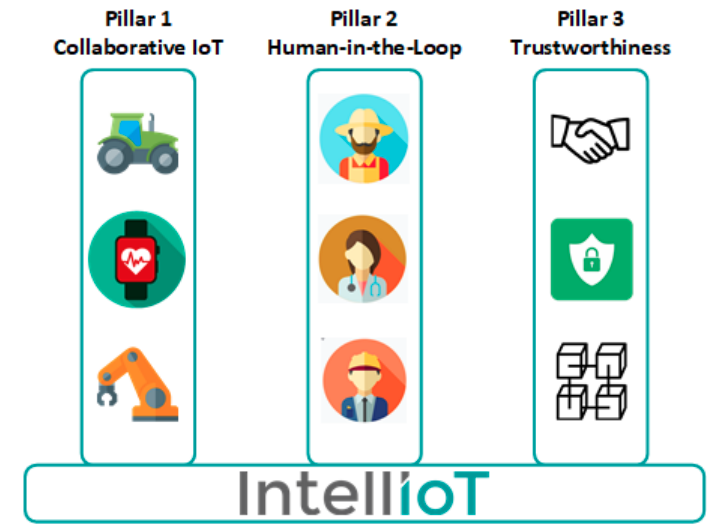
\includegraphics[width=0.8\linewidth]{images/intelliot-pillars.png}
    \caption{The three pillars of \textit{IntellIoT}.}
    \label{fig:intelliot-pillars}
\end{figure}

\subsection{Use Cases}
The above three key component areas are supported by \textit{IntellIoT}'s dynamically managed network and computation infrastructure that, combined, provide resource and edge management, orchestration capabilities, and network choreography, exploiting cutting-edge technologies like 5G.
Moreover, for the pillars to not remain only abstract concepts, various use cases that aim to address real-life problems in three core sectors were developed:

\begin{itemize}
    \item \textbf{Agriculture}: the application of IoT in agriculture could be a life-changer for humanity as we now witness how extreme weather, deteriorating soil, dry lands, and collapsing ecosystems make food production more and more complicated and expensive, not to mention the population growth that increases the demand for resources.
    Although ``smart farming'' is already a thing, \textit{IntellIoT} aims to bring it to the next level thanks to autonomous devices such as self-driving tractors and drones endowed with sensors and actuators.
    However, even though machines perform potentially dangerous, tiring, and repetitive tasks for humans, the latter still play a crucial role in managing the farm.
    Indeed, they can remote control the devices in uncertain situations, refining the Artificial Intelligence models.
    Additionally, human operators are in charge of defining the goals of the farming system, leveraging their experience and knowledge about the domain.
    \item \textbf{Healthcare}: IoT is revolutionizing the healthcare industry, mainly due to remote patient monitoring.
    Indeed, being endowed with specific sensors, devices can track the latter's vital signs and other health metrics and send the collected data to healthcare providers.
    Some examples of such devices are \textit{Continuous Glucose Monitoring} \cite{facchinetti2013real} and \textit{Dissolvable Brain Swelling}\cite{kang2016bioresorbable} sensors or ordinary smartwatches.
    This process improves the patient's quality of life, which does not need to be limited to their home or the hospital and can thus carry on with their regular everyday activities.
    Moreover, continuous monitoring and real-time data sharing allow timely interventions when necessary, and automatic data collection can drastically decrease the time and effort required to retrieve and manage information about the patient.
    Not to mention the opportunities for data analysis and possible Artificial Intelligence models that would support clinicians in being more efficient.
    However, this workflow potentially exposes patients' sensitive information; therefore, we find privacy, security, and trust assurance among the main focuses of \textit{IntellIoT} regarding this use case.
    \newline
    \item \textbf{Manufacturing}: IoT is one of the core driving forces behind Industry 4.0, which aims to digitalize and automate operational processes counting on as little support as possible from human operators, from the order submission to the delivery of the product.
    Leveraging AI and Machine Learning, robotics, and data analysis, IntellIoT envisions a future with shared manufacturing plants and multiple customers utilizing manufacturing as-a-service.
    According to the latter scenario, an intelligent IoT environment would derive a production plan from data received from a customer and select the appropriate machines for the planned steps.
    However, whenever AI is not sufficiently confident about a step, a human-in-the-loop can take over control remotely, providing information that will be learned by the Machine Learning algorithm thanks to continual learning.
\end{itemize}

\section{Domain-Expert Programming}
As already discussed, the crucial role of end-users in the definition of autonomous systems, the importance of their intervention in case of need, and their expertise are utterly unmatched by Artificial Intelligence algorithms and probably will be for a long time.

On top of that, the gap between programmers and end-users regarding domain comprehension is a well-acknowledged issue concerning software development.
Indeed, developers' poor understanding of the domain often results in projects missing their schedules or exceeding their budget, poor-quality software, or even wrong functionalities \cite{5089292}.
To address this critical issue, several techniques have been developed.
For instance, one of the core aspects of Domain Driven Design is \textit{knowledge crunching}, which aims to extract domain knowledge from the experts to reflect it in the code during the subsequent development phases.

On the other hand, a different approach might be taken directly involving domain experts in the programming process.
This kind of user can be defined as professionals in some domain different from computer science who need to use computers in their daily work and often have real needs to perform some programming activities that result in the creation or modification of software artifacts \cite{costabile2003domain}.
Given the latter definition and the premise suggesting the importance of domain expertise, providing domain experts with tools, such as domain-specific languages (DSL) or more user-friendly visual tools, that allow them to ``code'' or configure parts of complex systems feels very natural.
Therefore the need for an intuitive development environment in which users with no proper computer science background can naturally and seamlessly transform their domain knowledge into specifications with low-code (or possibly no-code).

\section{Proposing a Visual Programming Paradigm for Organizations}
Multi-Agent Systems is one of the core enabling technologies of the infrastructure of \textit{IntellIoT}.
MAS fit IoT because they tackle the complexity and handle the decentralization of the IoT ecosystem by providing a framework for coordinating the actions of a large number of devices, allowing the latter to communicate and make decisions toward the achievement of a common goal.
Another critical advantage of MAS is their ability to deal with partial knowledge, incomplete and imperfect information, and adapt and reason in real-time, which is crucial in dynamic, uncertain, open, and distributed networks.

However, the high-level expertise required to program agent-based systems hinders the large-scale adoption of MAS.
Thus, efforts have been made to eliminate the entry barrier to MAS development, such as creating an agent-oriented programming paradigm \cite{burattini2022agent}, which enables individuals without coding experience, but with knowledge of specific target domains, to design and (re)configure autonomous software.

Nevertheless, although this block-based visual development environment is suitable for defining single entities, a level of abstraction to handle the relations among and coordination of the latter is still missing.
Even though these aspects could be technically represented and managed directly in the mind of the agents, the adoption of adequate abstractions makes the solution dramatically more straightforward and elegant. \cite{boissier2020multi}

Therefore, the idea is to design and implement a visual language and a supportive development environment for MAS organizations, which is a novelty to our knowledge.
The core thesis work will be based on studying the existing organization models, with particular attention to the $\mathcal{M}\text{\footnotesize{OISE}}^{+}$ model, and developing an appropriate representation that could provide a suitable tradeoff between the expressiveness of code-based specifications and the ease of use of graphic programming interfaces.
A qualitative evaluation is also planned to receive feedback for the developed framework and to study how non-technical users solve problems by exploiting the visual language.

The following chapter provides an introduction to the background of the main technologies and research topics explored in the project.